\documentclass[tikz,border=3mm]{standalone}
% based on an answer by user http://tex.stackexchange.com/users/1952/ignasi
% on http://tex.stackexchange.com/questions/174317/creating-a-labeled-tetrahedron-with-tikzpicture
\begin{document}
\tikzset{>=latex}
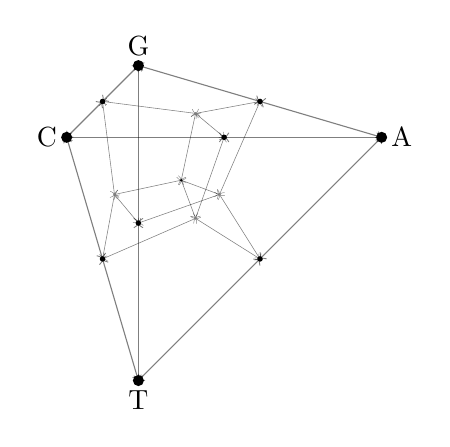
\begin{tikzpicture}[line join = round, line cap = round]
\pgfmathsetmacro{\xfactor}{1};
\pgfmathsetmacro{\yfactor}{1};
\pgfmathsetmacro{\zfactor}{1/sqrt(2)};
\coordinate [label=right:A] (A) at ( 2*\xfactor,  0*\yfactor, -2*\zfactor);
\coordinate [label=left:C]  (C) at (-2*\xfactor,  0*\yfactor, -2*\zfactor);
\coordinate [label=above:G] (G) at ( 0*\xfactor,  2*\yfactor,  2*\zfactor);
\coordinate [label=below:T] (T) at ( 0*\xfactor, -2*\yfactor,  2*\zfactor);

\coordinate [] (AC) at  ( 0*\xfactor,  0*\yfactor, -2*\zfactor);
\coordinate [] (AG) at  ( 1*\xfactor,  1*\yfactor,  0*\zfactor);
\coordinate [] (AT) at  ( 1*\xfactor, -1*\yfactor,  0*\zfactor);
\coordinate [] (CG) at  (-1*\xfactor,  1*\yfactor,  0*\zfactor);
\coordinate [] (CT) at  (-1*\xfactor, -1*\yfactor,  0*\zfactor);
\coordinate [] (GT) at  ( 0*\xfactor,  0*\yfactor, 2*\zfactor);

\coordinate [] (ACG) at  ( 0*\xfactor,  0.6666667*\yfactor, -0.6666667*\zfactor);
\coordinate [] (ACT) at  ( 0*\xfactor,  -0.6666667*\yfactor, -0.6666667*\zfactor);
\coordinate [] (AGT) at  ( 0.6666667*\xfactor,  0*\yfactor, 0.6666667*\zfactor);
\coordinate [] (CGT) at  ( -0.6666667*\xfactor,  0*\yfactor, 0.6666667*\zfactor);
\coordinate [] (ACGT) at  ( 0*\xfactor,  0*\yfactor, 0*\zfactor);


\draw[<->, opacity=.5] (A) -- (AC);
\draw[<->, opacity=.5] (AC) -- (C);
\draw[<->, opacity=.5] (A) -- (AG);
\draw[<->, opacity=.5] (AG) -- (G);
\draw[<->, opacity=.5] (A) -- (AT);
\draw[<->, opacity=.5] (AT) -- (T);
\draw[<->, opacity=.5] (C) -- (CG);
\draw[<->, opacity=.5] (CG) -- (G);
\draw[<->, opacity=.5] (C) -- (CT);
\draw[<->, opacity=.5] (CT) -- (T);
\draw[<->, opacity=.5] (G) -- (GT);
\draw[<->, opacity=.5] (GT) -- (T);


\draw[<->, opacity=.5, very thin] (AC) -- (ACG);
\draw[<->, opacity=.5, very thin] (AG) -- (ACG);
\draw[<->, opacity=.5, very thin] (CG) -- (ACG);

\draw[<->, opacity=.5, very thin] (AC) -- (ACT);
\draw[<->, opacity=.5, very thin] (AT) -- (ACT);
\draw[<->, opacity=.5, very thin] (CT) -- (ACT);

\draw[<->, opacity=.5, very thin] (AG) -- (AGT);
\draw[<->, opacity=.5, very thin] (AT) -- (AGT);
\draw[<->, opacity=.5, very thin] (GT) -- (AGT);

\draw[<->, opacity=.5, very thin] (CG) -- (CGT);
\draw[<->, opacity=.5, very thin] (CT) -- (CGT);
\draw[<->, opacity=.5, very thin] (GT) -- (CGT);


\draw[<->, opacity=.5, very thin] (ACG) -- (ACGT);
\draw[<->, opacity=.5, very thin] (ACT) -- (ACGT);
\draw[<->, opacity=.5, very thin] (AGT) -- (ACGT);
\draw[<->, opacity=.5, very thin] (CGT) -- (ACGT);


\foreach \i in {ACGT}
    \fill [black] (\i) circle (.5pt);

\foreach \i in {ACG, ACT, AGT, CGT}
    \fill [gray] (\i) circle (.5pt);

\foreach \i in {AC,AG,AT,CG,CT,GT}
    \fill [black] (\i) circle (1pt);
\foreach \i in {A,C,G,T}
    \fill [black] (\i) circle (2pt);

\end{tikzpicture}

\end{document}

% AXES
%\draw[->] (0,0) -- (3,0,0) node[right] {$x$};
%\draw[->] (0,0) -- (0,3,0) node[above] {$y$};
%\draw[->] (0,0) -- (0,0,3) node[below left] {$z$};
